\chapter{Resultados e discussões}

Como tanto para a programação no \emph{Google App Engine} como para o \emph{Android} a linguagem utilizada é \emph{Java} e portanto seu código é executado pela maquina virtuali \emph{java}. Adotou-se a ideia de se criar os dois \emph{softwares} em um ambiente \emph{desktop} padrão para depois portar, sem maiores problemas, para seus respectivos ambientes.\\

 Como  já explicado, foi utilizado uma metodologia de desenvolvimento baseado em \emph{scrum} com \emph{sprints}, que são intervalos de tempo definidos para pequenas implementações, variando de uma a duas semanas. Durante o tempo disponível para o desenvolvimento deste sistema, foi possível realizar seis \emph{sprints} e com isto implementar o funcionamento básico com alguns poucos comandos.\\

 Foram criados programas no paradigma cliente-servidor que comunicam-se através de \emph{sockets}, ambos os programas respeitando o padrão \emph{command} e o paradigma de computação orientada a objetos conhecido como \emph{open-closed principle}, que nos diz que entidades de software (módulos,classes e métodos) devem sempre ser abertos para extensão e fechados para modificações. Desta maneira, uma vez que a estrutura básica está criada, resta apenas incluir novos comandos que resultam em novas utilidades para o sistema, o que não será difícil uma vez que o sistema foi desenvolvido pensando em extensão.\\

\newpage 
Com o intuito de mostrar a evolução do sistema, o seguinte diagrama de classe da \emph{uml}\footnote{Unified Modeling Language} se faz útil:\\

\begin{figure}[h]
    \includegraphics[scale=0.35]{img/diagrama_class2.png}\\
    \caption{\it Diagrama de classe do sistema}
\end{figure}

Observando o diagrama, pode-se perceber a facilidade quanto a inserção de novas funcionalidades, pois para adicionar um novo comando, basta que este novo comando implemente a classe \emph{command} com sua própria interpretação de \emph{executa()}. Outro ponto interessante pode ser notado no fato de que o canal de comunicação é abstraído pela classe \emph{Canal}. Desta maneira caso seja necessário trocar a forma de comunicação atual, somente está classe será alterada.
 
\newpage
Quanto a funcionalidade, temos um exemplo em que um celular envia um comando perguntando qual é o tipo do seu interlocutor:\\
 \begin{figure}[h]
    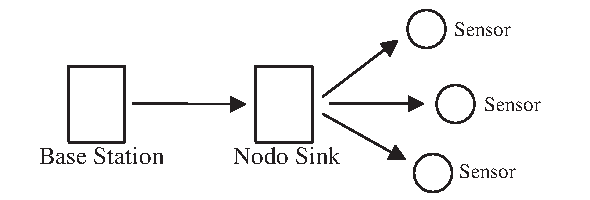
\includegraphics[scale=0.35]{img/exemplo.png}\\
    \caption{\it Exemplo de envio de comando}
\end{figure}


